%%%%%%%%%%%%%%%%%%%%%%%%%%%%%%%%%%%%%%%%%
% Short Sectioned Assignment
% LaTeX Template
% Version 1.0 (5/5/12)
%
% This template has been downloaded from:
% http://www.LaTeXTemplates.com
%
% Original author:
% Frits Wenneker (http://www.howtotex.com)
%
% License:
% CC BY-NC-SA 3.0 (http://creativecommons.org/licenses/by-nc-sa/3.0/)
%
%%%%%%%%%%%%%%%%%%%%%%%%%%%%%%%%%%%%%%%%%

%----------------------------------------------------------------------------------------
%	PACKAGES AND OTHER DOCUMENT CONFIGURATIONS
%----------------------------------------------------------------------------------------

\documentclass[paper=a4, fontsize=11pt]{scrartcl} % A4 paper and 11pt font size

\usepackage[T1]{fontenc} % Use 8-bit encoding that has 256 glyphs
\usepackage{fourier} % Use the Adobe Utopia font for the document - comment this line to return to the LaTeX default
\usepackage[english]{babel} % English language/hyphenation
\usepackage{amsmath,amsfonts,amsthm} % Math packages

\usepackage{graphicx}

\usepackage{sectsty} % Allows customizing section commands
\allsectionsfont{\centering \normalfont\scshape} % Make all sections centered, the default font and small caps

\usepackage{fancyhdr} % Custom headers and footers
\pagestyle{fancyplain} % Makes all pages in the document conform to the custom headers and footers
\fancyhead{} % No page header - if you want one, create it in the same way as the footers below
\fancyfoot[L]{} % Empty left footer
\fancyfoot[C]{} % Empty center footer
\fancyfoot[R]{\thepage} % Page numbering for right footer
\renewcommand{\headrulewidth}{0pt} % Remove header underlines
\renewcommand{\footrulewidth}{0pt} % Remove footer underlines
\setlength{\headheight}{13.6pt} % Customize the height of the header

\numberwithin{equation}{section} % Number equations within sections (i.e. 1.1, 1.2, 2.1, 2.2 instead of 1, 2, 3, 4)
\numberwithin{figure}{section} % Number figures within sections (i.e. 1.1, 1.2, 2.1, 2.2 instead of 1, 2, 3, 4)
\numberwithin{table}{section} % Number tables within sections (i.e. 1.1, 1.2, 2.1, 2.2 instead of 1, 2, 3, 4)

\setlength\parindent{0pt} % Removes all indentation from paragraphs - comment this line for an assignment with lots of text

%----------------------------------------------------------------------------------------
%	TITLE SECTION
%----------------------------------------------------------------------------------------

\newcommand{\horrule}[1]{\rule{\linewidth}{#1}} % Create horizontal rule command with 1 argument of height

\title{	
\normalfont \normalsize 
\textsc{BRSU} \\ [25pt] % Your university, school and/or department name(s)
\horrule{0.5pt} \\[0.4cm] % Thin top horizontal rule
\huge Neural Networks - Assignment 1 \\ % The assignment title
\horrule{2pt} \\[0.5cm] % Thick bottom horizontal rule
}

\author{Bastian Lang} % Your name

\date{\normalsize\today} % Today's date or a custom date

\begin{document}

\maketitle % Print the title

\section{Outline Chapter I}
\begin{itemize}
\item What is a neural network?

\begin{itemize}
\item Motivated by human brain
\item complex, nonlinear, parallel
\item Benefits of neural networks

\begin{itemize}
\item Nonlinearity
\item Input-output mapping
\item Adaptivity
\item Evidential Response
\item Contextual information
\item Fault tolerance
\item VLSI implementability
\item Uniformity of analysis and design
\item Neurobiological analogy
\end{itemize}

\end{itemize}

\item Human brain

\begin{itemize}
\item about 10 billion neurons
\item about 60 trillion synapses/connections
\item energetic efficient
\item chemical synapses: electrical signal $->$ chemical signal $->$ electrical signal
\item plasticity via new connections and modification of existing ones
\item structural level of organization

\end{itemize}

\item Models of a neuron

\begin{itemize}
\item Neuron: Information-processing unit
\item Three basic elements:
\begin{itemize}
\item Set of synapses
\item Adder
\item Activation function/squashing function
\end{itemize}

\item Types of activation function
\begin{itemize}
\item Threshold function (McCulloch-Pitts model)
\item Piecewise-linear function
\item Sigmoid function
\end{itemize}

\item Stochastic model of a neuron
\end{itemize}

\item Neural Networks viewed as directed graphs
\begin{itemize}
	\item Block diagram: functional description
	\item Signal-flow graph: signal flow
	\begin{itemize}
		\item Rule1: Signal flows in direction defined by arrow
		\item Rule2: Node signal equals sum of entering signals
		\item Rule3: Signal of node is transmitted to each outgoing link
	\end{itemize}
	\item Architectural graph: network layout
\end{itemize}

\item Feedback
	\begin{itemize}
		\item Feedback: Output influences input
		\item Recurrent networks
		\item closed-loop operator: $\frac{A}{1-AB}$
		\item open-loop operator: $AB$
	\end{itemize}

\item Network architectures
	\begin{itemize}
		\item Single-layer feedforward networks
		\begin{itemize}
			\item No hidden layer
		\end{itemize}
		\item Multi-layer feedforward networks
		\begin{itemize}
			\item Contains hidden layer
		\end{itemize}
		\item Recurrent Networks
		\begin{itemize}
			\item At least one feedback loop
		\end{itemize}
	\end{itemize}


\item Knowledge representation
\begin{itemize}
	\item Training via input-output pairs
	\item Learning: applying algorithm on a training set
	\item Generalization: test learned model on test set
	\item Rule1: Similar input from similar classes should be classified into the same category
	\item Rule2: Items of different classes should be given different representations in the network.
	\item Rule3: The more important a feature, the more neurons to represent it
	\item Rule4: Prior information should be built into the network beforehand
	\item How to build prior information into neural network design
	\begin{itemize}
		\item No well-defined rules
		\item receptive fields
		\item weight-sharing
	\end{itemize}
	\item How to build invariances into neural network design
	\begin{itemize}
		\item Invariance by structure
		\item Invariance by training
		\item Invariant feature space
	\end{itemize}
\end{itemize}

\item Artificial intelligence and neural networks
\begin{itemize}
	\item Representation
	\item Reasoning
	\item Learning
	\item Level of explanation
	\item Processing style
	\item Representational structure
\end{itemize}

\item Historical notes

\end{itemize}


\section{From Haykin's book, Chapter 1 problems - "Models of a neuron", solve any 2 out of 11
(1.1 to 1.11).}

\subsection{Exercise 1.6}
\textbf{Consider the pseudolinear activation function $\phi(v)$ shown in figure P1.6.\\
(a) Formulate $\phi(v)$ as a function of v.\\
(b) What happens to $\phi(v)$ if $\alpha$ is allowed to approach zero?}\\\\
 
(a)\\
\[ \phi(v) =
\left\{
	\begin{array}{ll}
		0  & \mbox{if } v < -0.5\alpha \\
		b & \mbox{if } v > 0.5\alpha \\
		\frac{b}{\alpha}v + 0.5b & \mbox{else}
	\end{array}
\right.\]\\\\

(b)\\
The function will not be defined for $\alpha =0$. The function becomes more and more similar to a step function with value 0 for $v<0$ and value b for $v>0$.

\subsection{Exercise 1.7}
\textbf{Repeat Problem 1.6 for the pseudolinear activation function $\phi(v)$ shown in Fig. P1.7.}\\\\

(a)\\
\[ \phi(v) =
\left\{
	\begin{array}{ll}
		-b  & \mbox{if } v < -\alpha \\
		b & \mbox{if } v > \alpha \\
		\frac{b}{\alpha}v & \mbox{else}
	\end{array}
\right.\]\\\\

(b)\\
The function will not be defined for $\alpha =0$. The function becomes more and more similar to a step function with value -b for $v<0$ and value b for $v>0$.

\section{From Haykin's book, Chapter 1 problems - "Network architectures", solve any 2 out of 7
(1.12 to 1.19) including 1.13.}

\subsection{Exercise 1.12}
\begin{figure}[ht]
	\centering
  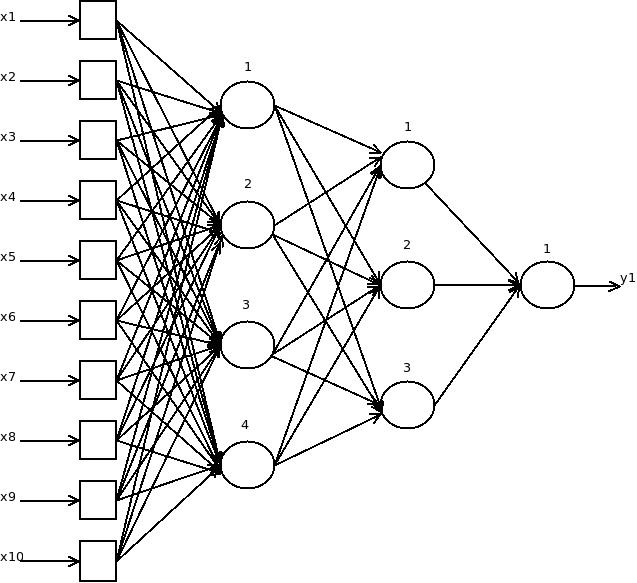
\includegraphics[width=0.5\textwidth]{1_12.jpeg}
	\caption{Fully recurrent network with five neurons, no self-feedback}
	\label{fig1}
\end{figure}


\subsection{Exercise 1.16}
\begin{figure}[ht]
	\centering
  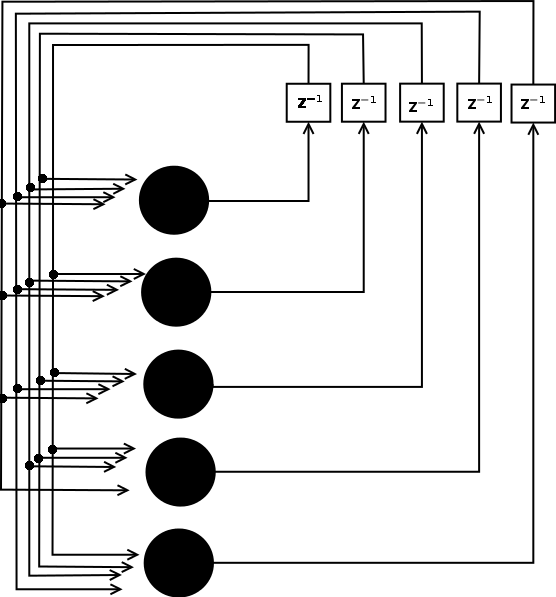
\includegraphics[width=0.5\textwidth]{1_16.png}
	\caption{Fully connected 10-4-3-1 feedforward network }
	\label{fig1}
\end{figure}

\end{document}